\documentclass{article} % For LaTeX2e
\usepackage{iclr2026_conference,times}

\input{math_commands.tex}

\usepackage{hyperref}
\usepackage{graphicx}
\usepackage{booktabs}
\usepackage{amsmath,amssymb}
\usepackage{microtype}
\usepackage{subcaption}
\usepackage{enumitem}
\usepackage{array}

\hypersetup{
  colorlinks=true,
  linkcolor=blue,
  citecolor=blue,
  urlcolor=blue
}

\iclrfinalcopy

\title{A Case Study of Staged Metric-Gated GRPO for Visual Numeric Reasoning}

% Keep the real author block in source; the ICLR style will hide it in review mode
% until \iclrfinalcopy is restored.
\author{Kunal Ghosh\\
Purdue University\\
West Lafayette, Indiana, USA\\
\texttt{ghosh178@purdue.edu}\\
\texttt{kg.aero@gmail.com}}

\newcommand{\mcell}[1]{\begin{tabular}[t]{@{}l@{}}#1\end{tabular}}

\begin{document}

\maketitle
\fancyhead{}
\lhead{}
\chead{}
\rhead{}

\begin{abstract}
We present a code-grounded case study of a staged metric-gated GRPO pipeline for visual numeric reasoning. The repository wraps \texttt{Qwen2.5-VL-7B-Instruct} with four main design choices: phase-wise curriculum over filtered MathVista subsets, a strict \texttt{<REASONING>} / \texttt{<SOLUTION>} response contract, a checkpoint-metric controller that preserves or raises structure-oriented reward weights when formatting or completion degrades, and alias-based checkpoint selection because later RL checkpoints are not always better. The report is intentionally narrow. Rather than claiming a new GRPO objective or a benchmark result, we analyze the archived artifacts that the repository itself produced during training and checkpoint selection. Under that internal evaluation protocol, the archived best large Phase C checkpoint and the archived best dedicated Phase D checkpoint each record exact match and tolerance accuracy of 0.75, up from 0.375 for a saved pre-refactor baseline snapshot, while maintaining parseability 1.0 and zero truncation on the monitored subset. The most important pattern in those artifacts is structure first, correctness later: smoke runs stabilize parseability and output form, and only then do larger continuation runs reach the 0.75 milestone. The contribution of the paper is therefore a reproducible case study of staged RL engineering for multimodal numeric QA, not a claim of broad empirical superiority.

\textbf{Code:} \url{https://github.com/kgaero/RL_GSPO_Qwen2.5VLM}
\end{abstract}

\section{Introduction}

Reinforcement-learning fine-tuning for language and vision-language models is often summarized as ``add reward, get better accuracy.'' In small multimodal projects, the reality is usually messier. Before correctness reward becomes informative, the policy must already emit outputs that are parseable, non-truncated, and structurally compatible with the evaluator. If those preconditions are unstable, RL updates can become difficult to interpret because an apparent correctness failure may in fact be a formatting or completion failure.

This paper studies one concrete repository that tackles that problem with staged metric-gated GRPO. The repository does not modify the GRPO loss itself. Instead, it builds a training stack around GRPO: filtered curriculum stages, a strict response contract, rule-based reward adaptation keyed to checkpoint metrics, and checkpoint aliases that allow continuation from the best structural or composite checkpoint rather than always from the most recent one. Our goal is to document what that stack does, what the saved artifacts say about it, and what kinds of claims the evidence can honestly support.

That framing makes this paper narrower than a conventional empirical method paper. We are not presenting a broad benchmark study, a new theorem, or a many-baseline comparison. We are presenting a repository case study. The value of that case study is that the code is unusually auditable for a small RL project: controller states are saved, checkpoint aliases are explicit, reward weights are persisted, and the main milestones are recoverable from repository artifacts. This makes the project a useful example of how staged RL can be organized when compute is limited and structural failures dominate early training.

Figure~\ref{fig:pipeline} summarizes the loop. A base VLM is prepared with LoRA adapters, trained on a stage-filtered phase mixture, evaluated checkpoint by checkpoint, and then fed back into a controller that adjusts the next segment's reward weights. Table~\ref{tab:stage-matrix} shows that the curriculum is implemented as overlapping filtered views over the same MathVista split rather than as disjoint datasets.

\paragraph{Case-study contributions.}
\begin{enumerate}[leftmargin=1.2em]
\item We document a staged GRPO training stack for visual numeric reasoning that explicitly separates structure stabilization from later correctness improvement.
\item We formalize the repository's metric-gated reward controller and checkpoint aliasing logic so they can be read as an auditable algorithm rather than as scattered implementation details.
\item We summarize the archived training trajectory that the repository itself used for continuation decisions, including the 0.75 exact-match milestone reached by the archived best large Phase C and dedicated Phase D checkpoints.
\item We clarify the scope of the evidence: these numbers are internal checkpoint-side measurements suitable for a reproducible case study, not a leaderboard-style claim.
\end{enumerate}

\begin{figure}[t]
\centering
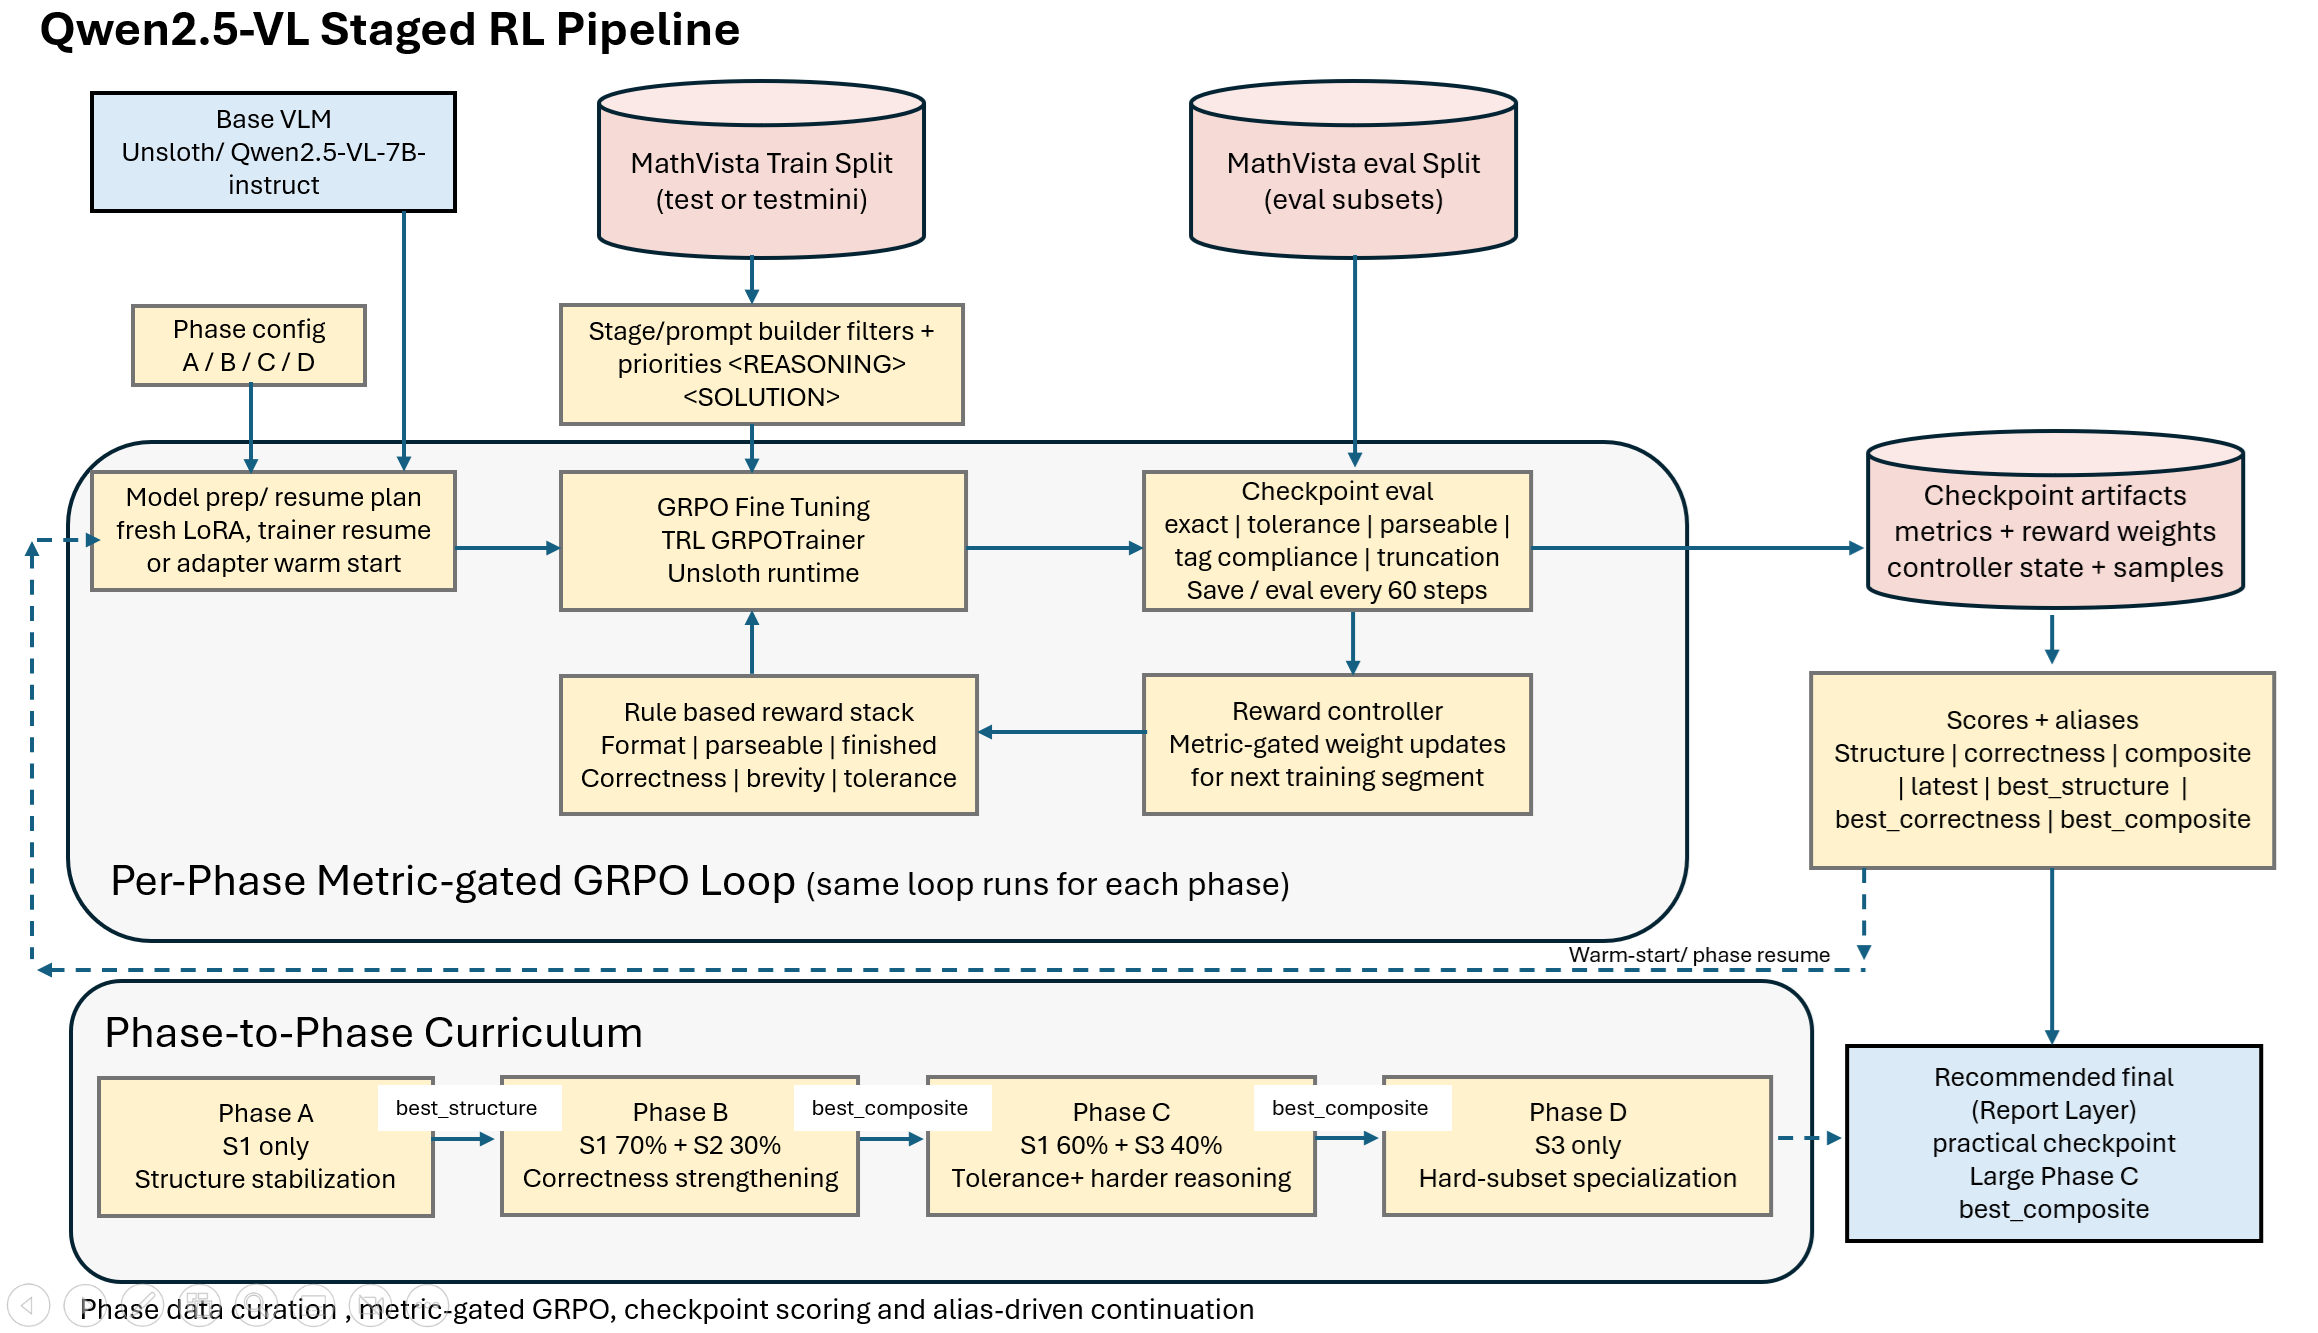
\includegraphics[width=\linewidth]{../../results/plots/staged_training_pipeline_better.png}
\caption{Overview of the repository's staged metric-gated GRPO loop. The pipeline couples phase-specific data curation, GRPO fine-tuning, checkpoint-side evaluation, reward-weight adaptation, and alias-based continuation. The contribution analyzed here is the training stack around GRPO rather than a new GRPO loss.}
\label{fig:pipeline}
\end{figure}

\section{Related Work}

\paragraph{RL fine-tuning and preference optimization.}
Recent RLHF and preference-optimization work has primarily focused on new objectives or more efficient learning regimes. DeepSeekMath introduced GRPO as a group-relative alternative to PPO for mathematical reasoning \citep{deepseekmath2024}. At ICLR 2025, SPPO proposed a self-play preference objective with a stronger theoretical framing than pairwise preference losses \citep{wu2025sppo}, while Asynchronous RLHF studied speed-quality trade-offs in off-policy online RLHF \citep{noukhovitch2025async}. Our paper is orthogonal to those contributions. We do not alter the underlying GRPO objective; we study how one repository wraps GRPO with curriculum, metric-gated reward scheduling, and checkpoint-selection logic in a failure-prone multimodal setting.

\paragraph{Multimodal mathematical reasoning.}
MathVista exposed the difficulty of mathematical reasoning in visual contexts and remains a useful benchmark for diagram, chart, table, and numeric QA behavior \citep{lu2024mathvista}. More recent ICLR papers have attacked that problem with larger synthetic corpora, progressive curricula, or more explicit visual reasoning mechanisms \citep{zhang2025mavis,qi2025cogcom}. Our scope is narrower. We do not introduce a new dataset or a new multimodal reasoning architecture. Instead, we analyze how a standard pretrained VLM behaves under a staged RL wrapper that prioritizes structural reliability before harder correctness pressure.

\paragraph{Curriculum and adaptive reward control.}
The repository is closest in spirit to curriculum and adaptive-control approaches that treat training as a sequence of regimes rather than as one stationary objective. The distinctive feature here is the granularity of adaptation: checkpoint metrics trigger reward changes directly. That makes the controller easy to audit, which is especially useful in a case-study setting where interpretability of the training loop matters as much as the raw score.

\section{Problem Setup and Design Goals}

We study a policy $\pi_\theta(c \mid x)$ that maps a visual question-answering input $x$ to a completion $c$. The repository does not treat success as a single scalar notion of accuracy. Instead, it decomposes success into a sequence of preconditions:
\begin{enumerate}[leftmargin=1.2em]
\item the model must emit the required tagged structure,
\item the final answer must be parseable,
\item the answer must finish within the completion budget, and
\item the parsed answer must be correct under exact or tolerance-based matching.
\end{enumerate}
The practical question is therefore not only how to optimize correctness, but when correctness reward becomes worth emphasizing. If structure is unstable, correctness reward is sparse and often misleading because malformed or truncated outputs never reach a meaningful matching stage.

The implementation makes three concrete design choices.
\begin{itemize}[leftmargin=1.2em]
\item \textbf{Easy-to-hard data staging.} The policy first sees easier integer-valued numeric problems before harder float and geometry-heavy subsets are emphasized.
\item \textbf{Metric-gated rewards.} Reward weights change only after checkpoint evaluation, using measured failure modes rather than a fixed epoch schedule.
\item \textbf{Alias-based continuation.} Checkpoint continuation is based on structure, correctness, or composite aliases rather than assuming the latest checkpoint is best.
\end{itemize}
These choices are modest in isolation, but together they define the engineering story of the repository.

\section{Method}

\subsection{Task, response contract, and phase structure}

The code targets MathVista-style visual question answering in which the answer is primarily numeric and free-form. Each prompt is wrapped with a strict output contract:
\begin{quote}
\small\ttfamily
<REASONING> ... </REASONING>\\
<SOLUTION> single numeric answer </SOLUTION>
\end{quote}
This contract matters because both the reward functions and the evaluator depend on extracting a unique solution string from the completion. The pipeline also contains a separate multi-choice scaffold, but that branch is disabled by default and is not part of the main case-study evidence.

The curriculum is organized into stages and phases. Stages are filtered subsets over the same dataset. In the default configuration:
\begin{itemize}[leftmargin=1.2em]
\item \textbf{Stage 1} restricts to easier English free-form integer questions on synthetic scenes, tables, and natural images.
\item \textbf{Stage 2} broadens to integer and float answers, adding tables, charts, plots, and scientific figures.
\item \textbf{Stage 3} emphasizes harder geometry, scientific-figure, plot, and abstract-scene problems.
\end{itemize}
Phases then mix these stages with different reward emphases:
\begin{itemize}[leftmargin=1.2em]
\item \textbf{Phase A}: Stage 1 only, structure stabilization.
\item \textbf{Phase B}: $0.7$ Stage 1 + $0.3$ Stage 2, early correctness strengthening.
\item \textbf{Phase C}: $0.6$ Stage 2 + $0.4$ Stage 3, harder reasoning and tolerance reward.
\item \textbf{Phase D}: Stage 3 only, hard-subset specialization with a longer completion budget.
\end{itemize}

\begin{table}[t]
\centering
\setlength{\tabcolsep}{2pt}
\renewcommand{\arraystretch}{1.12}
\scriptsize
\begin{tabular}{>{\raggedright\arraybackslash}p{0.14\linewidth}>{\raggedright\arraybackslash}p{0.27\linewidth}>{\raggedright\arraybackslash}p{0.27\linewidth}>{\raggedright\arraybackslash}p{0.27\linewidth}}
\hline
\textbf{Filter} & \textbf{S1 Easy Numeric} & \textbf{S2 Medium / Float} & \textbf{S3 Hard Numeric} \\
\hline
Stage ID & \texttt{stage1\_easy\_numeric} & \texttt{stage2\_float\_numeric} & \texttt{stage3\_hard\_numeric} \\
\hline
Goal & easy numeric stabilization & moderate precision and broader numeric coverage & harder multistep numeric reasoning \\
\hline
Question type & \texttt{free\_form} & \texttt{free\_form} & \texttt{free\_form} \\
\hline
Answer type & \texttt{integer} & \texttt{integer}, \texttt{float} & \texttt{integer}, \texttt{float} \\
\hline
Language & \texttt{english} & \texttt{english} & \texttt{english} \\
\hline
Answer mode & \texttt{numeric\_free\_form} & \texttt{numeric\_free\_form} & \texttt{numeric\_free\_form} \\
\hline
Context families & \mcell{\texttt{synthetic scene}\\\texttt{table}\\\texttt{natural image}} & \mcell{\texttt{table}\\\texttt{chart}\\\texttt{plot}\\\texttt{scientific figure}\\\texttt{natural image}} & \mcell{\texttt{geometry diagram}\\\texttt{plot}\\\texttt{scientific figure}\\\texttt{abstract scene}} \\
\hline
Skills (any) & \mcell{\texttt{arithmetic reasoning}\\\texttt{statistical reasoning}\\\texttt{numeric commonsense}} & \mcell{\texttt{arithmetic reasoning}\\\texttt{statistical reasoning}\\\texttt{scientific reasoning}\\\texttt{numeric commonsense}} & \mcell{\texttt{geometry reasoning}\\\texttt{algebraic reasoning}\\\texttt{scientific reasoning}\\\texttt{arithmetic reasoning}\\\texttt{statistical reasoning}} \\
\hline
Hard only & False & False & True \\
\hline
Priority bias & \mcell{ctx: synthetic scene\\ctx: table\\skills: arithmetic reasoning\\skills: statistical reasoning\\skills: numeric commonsense\\grades: elementary school\\grades: daily life} & \mcell{ctx: table\\ctx: chart\\ctx: plot\\ctx: scientific figure\\skills: statistical reasoning\\skills: scientific reasoning\\skills: arithmetic reasoning} & \mcell{ctx: geometry diagram\\ctx: scientific figure\\ctx: plot\\skills: geometry reasoning\\skills: algebraic reasoning\\skills: scientific reasoning\\grades: high school\\grades: college} \\
\hline
\end{tabular}
\caption{Code-derived filter definitions for the three numeric curriculum stages used in the main training path. The stages overlap and are implemented as filtered views over the same MathVista split, not as fixed disjoint datasets.}
\label{tab:stage-matrix}
\end{table}

\subsection{Reward decomposition}

For a completion $c$, the repository computes six per-sample reward components:
\begin{equation}
R(c)=\sum_{j=1}^{6} w_j r_j(c),
\end{equation}
where the components correspond to \texttt{format}, \texttt{parseable}, \texttt{finished}, \texttt{correctness}, \texttt{brevity}, and \texttt{tolerance}. The initial weights are phase-specific. Phase A places relatively high weight on structure and completion; Phase C raises correctness and activates tolerance reward.

The implementation never allows structure rewards to decay fully to zero. That is the core design intuition of the repository: even when exact match becomes the main target, structure remains a necessary condition for receiving useful reward. The exact code-aligned reward definitions are reproduced in the supplement.

\subsection{Metric-gated reward control}

The reward controller updates weights after each checkpoint evaluation using explicit rules derived from observed metrics. Let $p$ denote parseable-answer rate, $s$ solution-tag compliance, $r$ reasoning-tag compliance, $m$ malformed rate, $t$ truncation rate, and $e$ exact match. The repository applies the following guards:
\begin{align}
p < 0.85 &\Rightarrow w_{\text{parseable}} \leftarrow \max(w_{\text{parseable}}, 0.75),\\
(s < 0.90)\ \vee\ (r < 0.88)\ \vee\ (m > 0.10) &\Rightarrow w_{\text{format}} \leftarrow \max(w_{\text{format}}, 0.75),\\
(t > 0.15)\ \vee\ (\bar{\ell} > 0.85L) &\Rightarrow w_{\text{finished}} \leftarrow w_{\text{finished}} + 0.25,
\end{align}
where $\bar{\ell}$ is average completion length and $L$ is the completion budget.

Correctness is escalated only when structure is already stable. Stability requires
\begin{equation}
p \ge 0.92,\quad s \ge 0.95,\quad r \ge 0.93,\quad m \le 0.05,\quad t \le 0.08,
\end{equation}
for a two-checkpoint window. If that condition holds and exact-match improvement over the window is below $0.02$, the controller increases correctness weight by $0.50$. All weights are then clamped to configured bounds. The rule set is intentionally simple enough to audit directly in saved checkpoint artifacts.

\subsection{Checkpoint-side evaluation and alias-based selection}

Instead of treating the most recent checkpoint as the default continuation point, the repository evaluates every saved checkpoint and computes three aggregate scores:
\begin{align}
S_{\text{struct}} &= 0.35\,p + 0.20\,s + 0.20\,r - 0.15\,m - 0.10\,t, \\
S_{\text{corr}} &= 0.70\,e + 0.20\,a_{\text{tol}} + 0.10\,p, \\
S_{\text{comp}} &= 0.45\,e + 0.15\,a_{\text{tol}} + 0.15\,p + 0.10\,s + 0.05\,r - 0.05\,m - 0.05\,t,
\end{align}
where $a_{\text{tol}}$ is tolerance accuracy. These scores back four aliases: \texttt{latest}, \texttt{best\_structure}, \texttt{best\_correctness}, and \texttt{best\_composite}. Cross-phase continuation typically resumes from \texttt{best\_structure} or \texttt{best\_composite}, while same-phase restarts may use full trainer resume from \texttt{latest}. This distinction matters in the repository because the code supports both full trainer-state restoration and LoRA-only warm start.

\section{Repository Setting and Archived Evaluation Protocol}

\paragraph{Dataset and model.}
The implementation targets the Hugging Face release of MathVista\footnote{\url{https://huggingface.co/datasets/AI4Math/MathVista}} and loads \texttt{Qwen2.5-VL-7B-Instruct}\footnote{\url{https://huggingface.co/Qwen/Qwen2.5-VL-7B-Instruct}} as the base VLM. For context we cite the MathVista benchmark paper \citep{lu2024mathvista} and the Qwen2.5-VL technical report \citep{bai2025qwen25vl}.

\paragraph{Runtime profile.}
The repository's main successful runs use the conservative \texttt{kaggle\_t4} profile: 4-bit loading, LoRA rank $8$, max sequence length $1280$, image size $336$, gradient accumulation $4$, two sampled generations per prompt during RL, max prompt length $320$, and max completion length $64$ (or $96$ in Phase D). The trainer uses TRL's \texttt{GRPOTrainer} with sequence-level importance sampling and \texttt{dr\_grpo} loss.

\begin{table}[t]
\centering
\setlength{\tabcolsep}{3pt}
\renewcommand{\arraystretch}{1.15}
\scriptsize
\begin{tabular}{>{\raggedright\arraybackslash}p{0.28\linewidth}>{\raggedright\arraybackslash}p{0.12\linewidth}>{\raggedright\arraybackslash}p{0.13\linewidth}>{\raggedright\arraybackslash}p{0.27\linewidth}>{\raggedright\arraybackslash}p{0.10\linewidth}}
\hline
\textbf{Parameter} & \textbf{Default} & \textbf{New Value} & \textbf{Function Name} & \textbf{Phase} \\
\hline
\mcell{\texttt{max\_seq\_length}} & 16384 & 1280 & \mcell{\texttt{FastVisionModel.}\\\texttt{from\_pretrained}} & all \\
\hline
\mcell{\texttt{image\_size}} & 512 & 336 & \mcell{\texttt{build\_stage\_dataset}} & all \\
\hline
\mcell{\texttt{gpu\_memory\_}\\\texttt{utilization}} & 0.8 & 0.65 & \mcell{\texttt{FastVisionModel.}\\\texttt{from\_pretrained}} & all \\
\hline
\mcell{LoRA config\\(\texttt{lora\_rank} / \texttt{max\_lora\_rank} /\\ \texttt{lora\_alpha})} & 16 / None / 16 & 8 / 8 / 8 & \mcell{\texttt{FastVisionModel.}\\\texttt{get\_peft\_model}} & all \\
\hline
\mcell{\texttt{compilation\_}\\\texttt{config}} & unset & \mcell{level 3\\PIECEWISE} & \mcell{\texttt{FastVisionModel.}\\\texttt{from\_pretrained}} & all \\
\hline
\mcell{Training budget\\(\texttt{gradient\_accumulation\_}\\\texttt{steps} /\\ \texttt{num\_generations})} & 2 / 4 & 4 / 2 & \mcell{\texttt{GRPOConfig}} & all \\
\hline
\mcell{Prompt budget\\(\texttt{max\_prompt\_length} /\\ \texttt{max\_completion\_length})} & 1024 / 256 & 320 / 64 & \mcell{\texttt{GRPOConfig}} & A--C, E \\
\hline
\mcell{Eval sampling\\(\texttt{num\_samples\_per\_prompt} /\\ \texttt{max\_eval\_examples\_}\\\texttt{per\_subset})} & 4 / None & 1 / 2 & \mcell{\texttt{SamplingParams}} & all \\
\hline
\mcell{Phase D completion budget\\(\texttt{max\_completion\_length})} & 320 & 96 & \mcell{\texttt{GRPOConfig} /\\\texttt{SamplingParams}} & D only \\
\hline
\end{tabular}
\caption{Code-derived implementation summary of the low-memory profile used by the archived successful runs. The \textbf{Function Name} column lists the concrete runtime method or config class that consumes the setting, rather than the config-builder that defines its default. The smoke experiments and the larger continuation therefore share the same Kaggle T4-safe operating regime.}
\label{tab:t4-profile}
\end{table}

\paragraph{Archived evaluation protocol and reporting choice.}
All quantitative values reported in this paper are taken from archived checkpoint-side artifacts generated during the original runs. Those archived values are the ones that the repository itself used for controller decisions and checkpoint aliasing. In smoke runs the code trains on \texttt{testmini} and also evaluates on \texttt{testmini}; in the larger continuation the code trains on \texttt{test} and evaluates on \texttt{testmini}. Under the Kaggle profile, evaluation uses one sampled completion per prompt and caps each subset at two examples. We therefore treat the numbers below as internal measurements for a reproducible repository case study, not as benchmark-comparable MathVista results.

\paragraph{Reproducibility.}
The repository saves checkpoint-side artifacts including metrics, subset metrics, reward weights, controller state, controller decision logs, prompt-level records, and sample-level JSONL traces. It also includes 26 unit tests covering configuration, data filtering, parsing, checkpointing, evaluation aggregation, controller behavior, and runtime compatibility.

\begin{table}[t]
\centering
\small
\caption{Archived milestone checkpoints under the repository's internal evaluation protocol. These are the saved checkpoint-side metrics used by the original continuation logic.}
\label{tab:milestones}
\begin{tabular}{lcccccc}
\toprule
Checkpoint & EM & Tol & Parse & Malf. & Trunc. & Comp. \\
\midrule
Pre-refactor baseline & 0.375 & 0.375 & 0.641 & 0.359 & 0.242 & 0.405 \\
Smoke Phase A best & 0.500 & 0.500 & 0.500 & 0.500 & 0.500 & 0.400 \\
Smoke Phase B best & 0.500 & 0.500 & 1.000 & 0.000 & 0.000 & 0.600 \\
Smoke Phase C best & 0.500 & 0.500 & 1.000 & 0.000 & 0.000 & 0.600 \\
Large Phase C best & \textbf{0.750} & \textbf{0.750} & \textbf{1.000} & \textbf{0.000} & \textbf{0.000} & \textbf{0.750} \\
Dedicated Phase D best & \textbf{0.750} & \textbf{0.750} & \textbf{1.000} & \textbf{0.000} & \textbf{0.000} & \textbf{0.750} \\
\bottomrule
\end{tabular}
\end{table}

\section{Archived Results}

\subsection{Structure improves before correctness in the archived trajectory}

Table~\ref{tab:milestones} shows the clearest pattern in the saved artifacts. The archived pre-refactor baseline snapshot reaches only $0.641$ parseability with $0.359$ malformed rate and $0.242$ truncation. Smoke Phase A shortens outputs, but structure remains poor. The decisive structural change appears in archived Smoke Phase B: parseability, reasoning-tag compliance, and solution-tag compliance all reach $1.0$, while malformed and truncation drop to zero. Exact match, however, remains at $0.5$. Within the repository's own training-time measurements, that is the crucial transition: structural reliability saturates before the main correctness gain arrives.

\begin{figure*}[p]
\centering
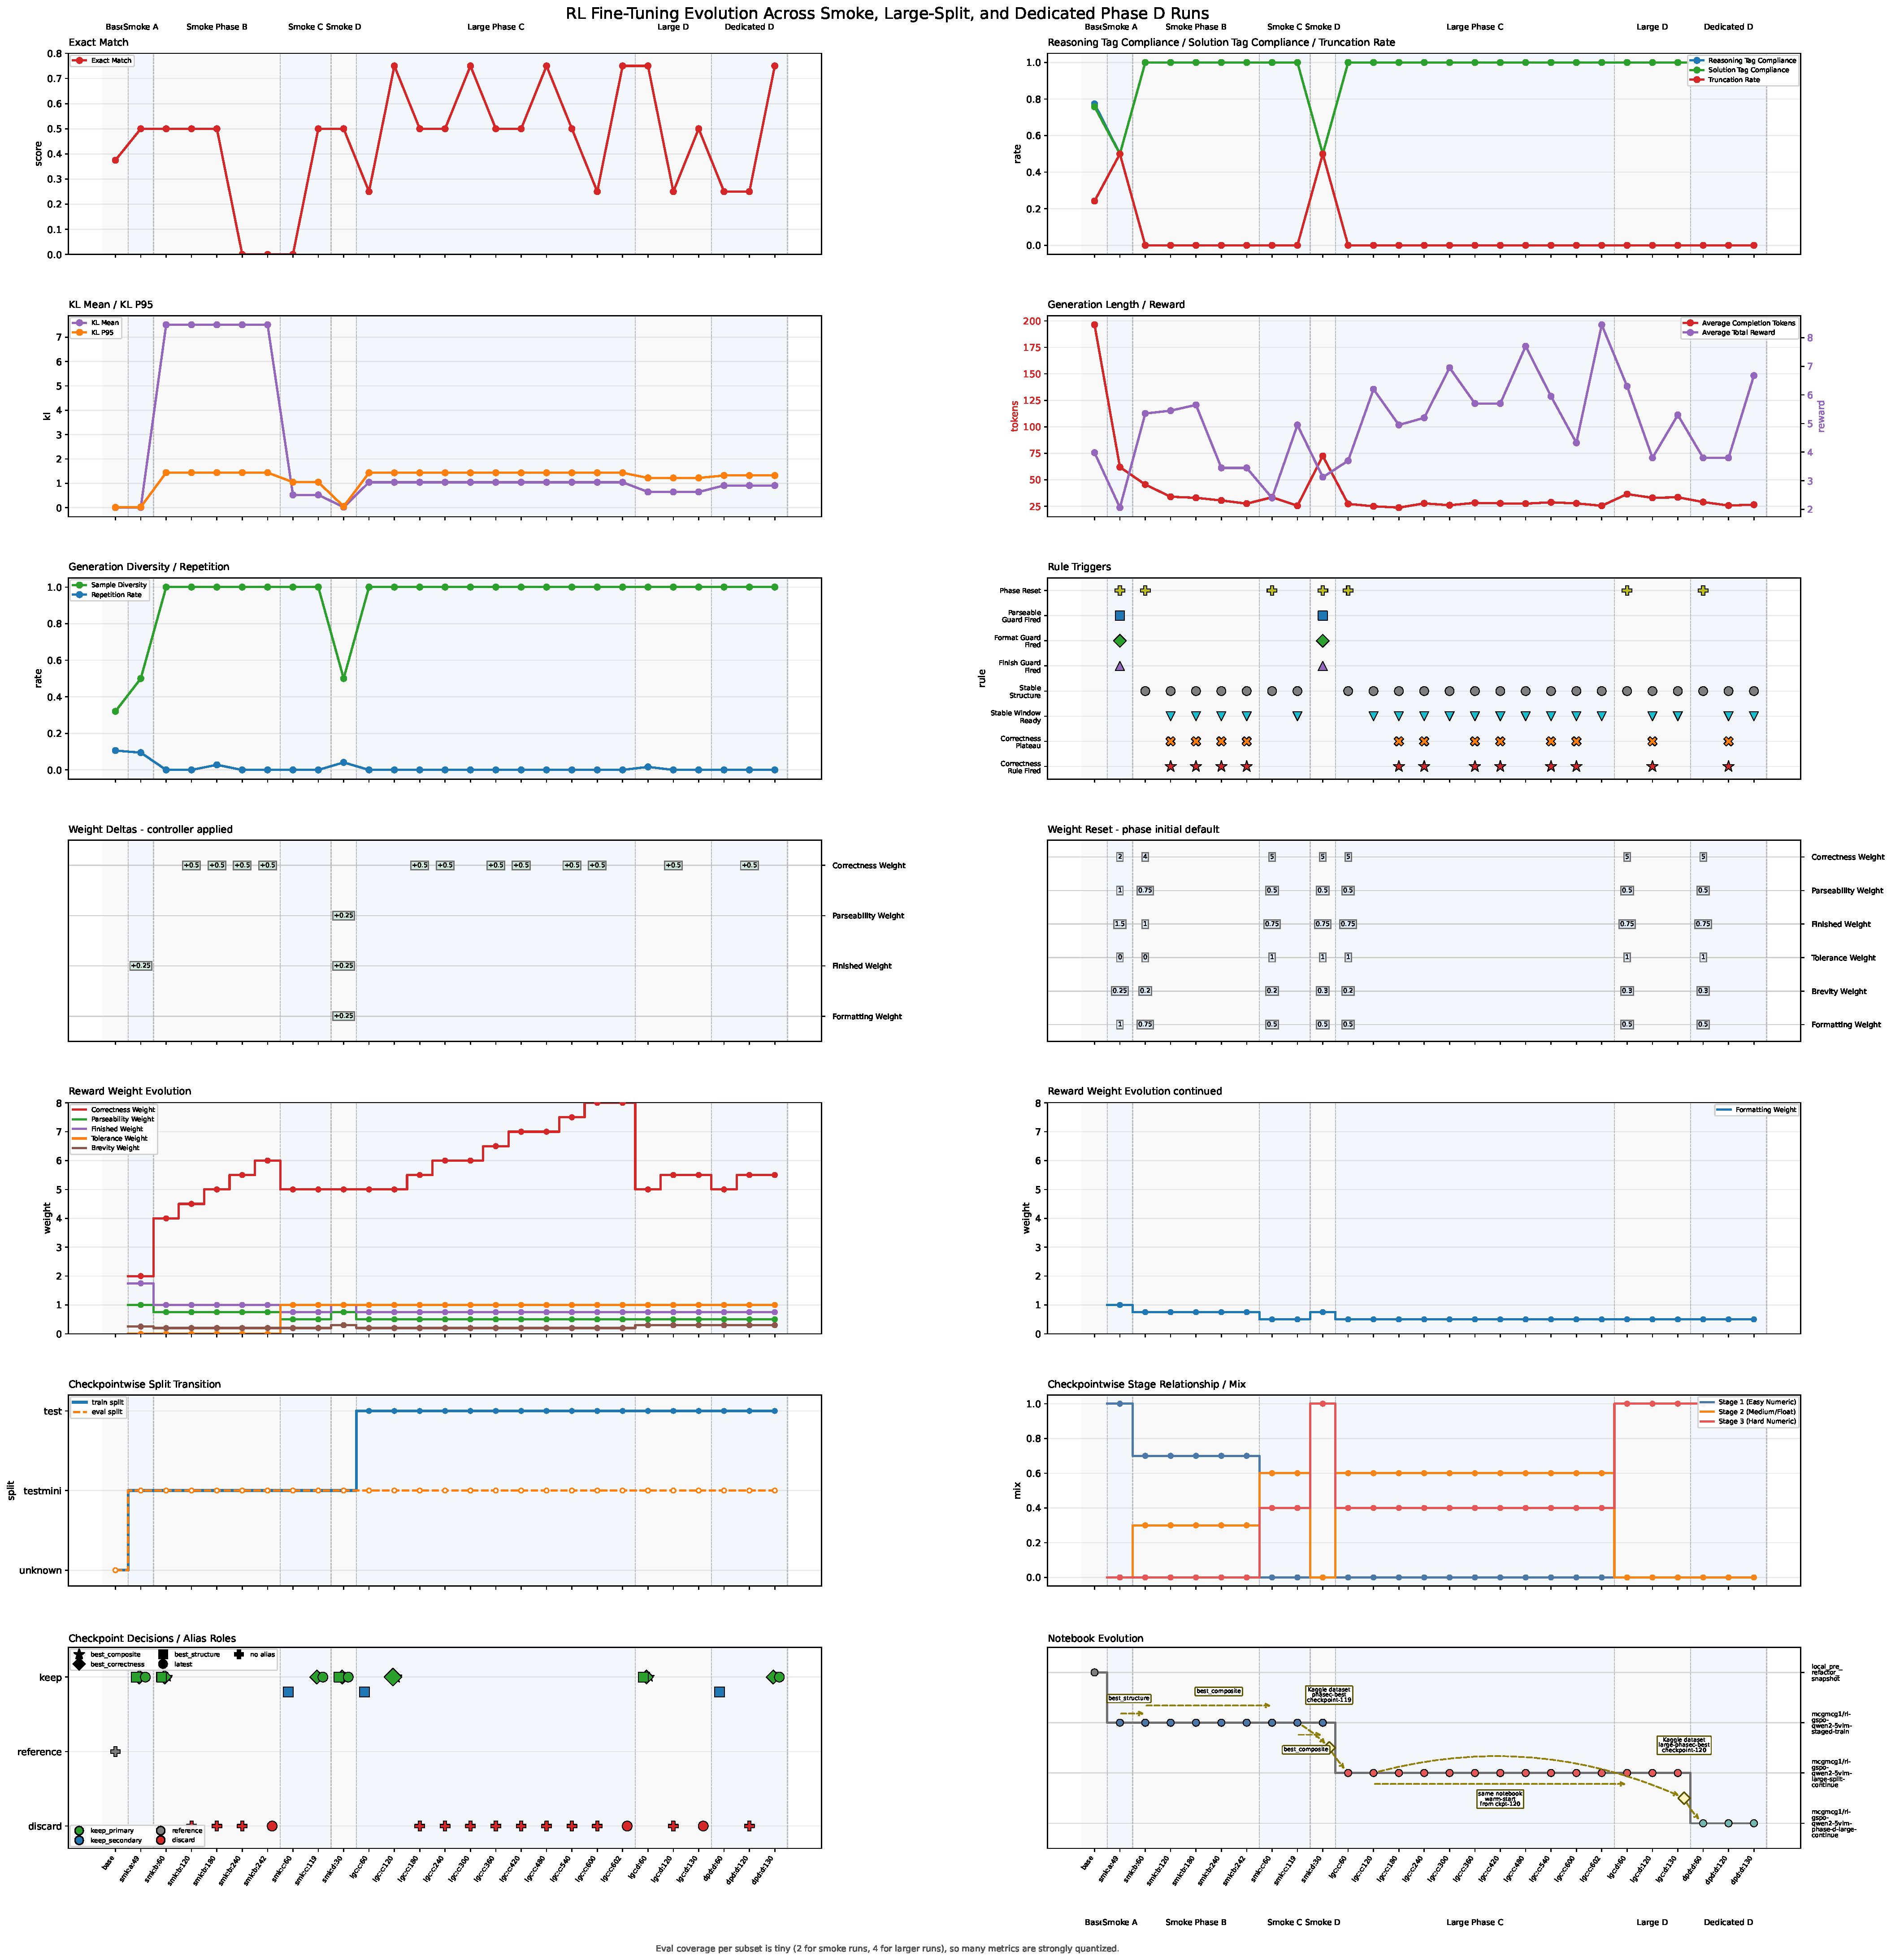
\includegraphics[width=\textwidth,height=0.9\textheight,keepaspectratio]{../../results/plots/evolution_panels_notebook_paper.pdf}
\caption{Training evolution across archived milestone checkpoints. The main qualitative pattern is structure first, correctness later: structural metrics stabilize by the smoke Phase B / Phase C regime, while the archived 0.75 exact-match milestone appears only after larger continuation.}
\label{fig:evolution}
\end{figure*}

Figure~\ref{fig:evolution} makes the transition visually explicit. Once structural metrics saturate, the archived trajectory stops looking like ``make outputs valid'' and starts looking like ``make valid outputs correct.'' That reading is consistent with the controller design: early checkpoints spend reward mass on formatting, parseability, and clean completion; later checkpoints inherit those gains and then receive more correctness pressure.

\subsection{The archived 0.75 milestone appears in larger continuation}

The strongest archived checkpoints in the repository are the large-split Phase C model at checkpoint 120 and the dedicated Phase D model at checkpoint 130. Relative to the saved baseline snapshot, the archived large Phase C checkpoint moves exact match from $0.375$ to $0.75$, tolerance accuracy from $0.375$ to $0.75$, parseability from $0.641$ to $1.0$, and average completion length from $196.3$ to $25.0$ tokens. Table~\ref{tab:base-final} summarizes that before-versus-after comparison.

\begin{table}[t]
\centering
\scriptsize
\setlength{\tabcolsep}{3pt}
\renewcommand{\arraystretch}{1.04}
\caption{Comparison between the saved pre-refactor baseline snapshot and the archived best large Phase C checkpoint. In this paper the table should be read as an outcome summary for the archived run artifacts, not as a benchmark table.}
\label{tab:base-final}
\begin{tabular*}{\linewidth}{@{\extracolsep{\fill}} p{0.50\linewidth} r r r @{}}
\toprule
\multicolumn{4}{@{}l@{}}{\textbf{Core Accuracy}} \\
\cmidrule(lr){1-4}
\textbf{Eval} & \textbf{Base} & \textbf{Trained} & \textbf{\% Improvement} \\
\midrule
\textbf{Exact Match} & \textbf{37.5\%} & \textbf{75.0\%} & \textcolor{green!50!black}{\textbf{+100.0\%}} \\
Tolerance Accuracy & 37.5\% & 75.0\% & \textcolor{green!50!black}{\textbf{+100.0\%}} \\
\midrule
\multicolumn{4}{@{}l@{}}{\textbf{Structure / Completion}} \\
\cmidrule(lr){1-4}
\textbf{Eval} & \textbf{Base} & \textbf{Trained} & \textbf{\% Improvement} \\
\midrule
Parseable Rate & 64.1\% & 100.0\% & \textcolor{green!50!black}{\textbf{+56.1\%}} \\
\textbf{Reasoning Tag Compliance} & \textbf{77.3\%} & \textbf{100.0\%} & \textcolor{green!50!black}{\textbf{+29.3\%}} \\
\textbf{Solution Tag Compliance} & \textbf{75.8\%} & \textbf{100.0\%} & \textcolor{green!50!black}{\textbf{+32.0\%}} \\
Well-Formed Rate & 64.1\% & 100.0\% & \textcolor{green!50!black}{\textbf{+56.1\%}} \\
\mcell{Malformed Rate\\(lower better)} & 35.9\% & 0.0\% & \textcolor{green!50!black}{\textbf{+100.0\%}} \\
Completion Success Rate & 75.8\% & 100.0\% & \textcolor{green!50!black}{\textbf{+32.0\%}} \\
\mcell{Truncation Rate\\(lower better)} & 24.2\% & 0.0\% & \textcolor{green!50!black}{\textbf{+100.0\%}} \\
\midrule
\multicolumn{4}{@{}l@{}}{\textbf{Generation}} \\
\cmidrule(lr){1-4}
\textbf{Eval} & \textbf{Base} & \textbf{Trained} & \textbf{\% Improvement} \\
\midrule
\mcell{Average Completion Tokens\\(lower better)} & 196.3 & 25.0 & \textcolor{green!50!black}{\textbf{+87.3\%}} \\
\mcell{Repetition Rate\\(lower better)} & 10.6\% & 0.0\% & \textcolor{green!50!black}{\textbf{+100.0\%}} \\
Sample Diversity & 32.0\% & 100.0\% & \textcolor{green!50!black}{\textbf{+212.2\%}} \\
\midrule
\multicolumn{4}{@{}l@{}}{\textbf{Scores / Reward}} \\
\cmidrule(lr){1-4}
\textbf{Eval} & \textbf{Base} & \textbf{Trained} & \textbf{\% Improvement} \\
\midrule
Average Total Reward & 3.98 & 6.2 & \textcolor{green!50!black}{\textbf{+55.7\%}} \\
Structure Score & 45.2\% & 75.0\% & \textcolor{green!50!black}{\textbf{+65.8\%}} \\
Correctness Score & 40.2\% & 77.5\% & \textcolor{green!50!black}{\textbf{+93.0\%}} \\
Composite Score & 40.5\% & 75.0\% & \textcolor{green!50!black}{\textbf{+85.0\%}} \\
\bottomrule
\end{tabular*}

\vspace{0.3em}
{\scriptsize\emph{Source:} Pre-Refactor Baseline (\texttt{base}) vs Large Phase C checkpoint-120 (\texttt{lgc:c:120}) from the repository's archived checkpoint tables.}
\end{table}

An important nuance is that the archived dedicated Phase D run matches, rather than exceeds, the archived best Phase C score. In other words, the case-study evidence supports hard-subset specialization as a viable continuation path, but it does not suggest that Stage-3-only specialization clearly dominates the mixed Stage 2/3 continuation.

\subsection{Archived checkpoints motivate alias-based selection}

The repository's saved runs also show why alias-based checkpoint selection was part of the implementation. In archived Smoke Phase B, the best composite checkpoint reaches exact match $0.5$ with perfect structure, while the latest checkpoint regresses to exact match $0.0$ despite keeping parseability and tag compliance at $1.0$. In the archived same-notebook Phase D branch, the best checkpoint reaches $0.75$ exact match but the latest checkpoint ends at $0.5$. This is not a theorem about RL in general. It is a concrete property of the observed checkpoint lineage in this repository, and it explains why the author introduced explicit aliases instead of resuming blindly from \texttt{latest}.

\subsection{The archived controller audit is consistent with the intended policy}

The saved controller audit covers 26 evaluated checkpoints across seven phase resets. Its main descriptive result is that the rules fire in the expected order. Parseability, formatting, and finish guards fire only twice each, concentrated in the structurally weak part of the trajectory. Correctness escalation fires 12 times, but only after structure is already stable. Notably, six of those correctness escalations happen on checkpoints where exact match has regressed rather than merely plateaued. In a case-study framing, that behavior is useful because it exposes the controller's bias directly: once structure is considered solved, the system responds to weak accuracy progress by increasing correctness pressure rather than by re-raising structure rewards.

The same combined view in Figure~\ref{fig:evolution} places that audit trail back into the checkpoint lineage. In the single-figure presentation, the controller-side panels remain available without splitting the narrative into separate quality and control figures.

\subsection{The same low-memory profile underlies the archived 0.75 result}

Table~\ref{tab:t4-profile} and the saved runtime-tuning tables make a second descriptive point clearer. The archived large continuation does not coincide with a more permissive hardware regime. The successful smoke and large-split runs share the same Kaggle T4 profile: sequence length $1280$ instead of $16384$, image size $336$ instead of $512$, LoRA rank $8$ instead of $16$, and two sampled generations instead of four. The cost is a shorter reasoning budget and lower generation diversity. The benefit is a stable single-GPU operating regime that supports both early curriculum validation and later continuation without changing the basic VRAM regime.

\section{Discussion}

The main value of this report is descriptive rather than universal. The repository suggests a layered story for one compute-constrained multimodal RL project.

First, a strict response contract makes structural failures measurable. Second, structure-oriented reward components give the optimizer a path to improve those failures before exact match is reliable. Third, a checkpoint-metric controller stops correctness reward from dominating too early. Fourth, alias-based checkpoint selection acknowledges that the saved trajectory is non-monotonic. Taken together, these choices turn the training loop into something that is easier to audit and reason about.

At the same time, the case-study framing imposes discipline on the claims. We do not claim that the archived 0.75 checkpoints establish a new state of the art. We do not claim that the controller is uniquely responsible for every improvement, because the repository does not contain the ablations required for that conclusion. The narrower claim is that the archived artifacts are internally consistent with a structure-first training recipe and that the implementation makes those dynamics unusually legible.

\section{Limitations and Reproducibility}

The limitations are substantial and should shape how the report is read.

\begin{itemize}[leftmargin=1.2em]
\item The reported numbers are archived checkpoint-side measurements from the original runs, not an external benchmark evaluation.
\item The monitored evaluation subset is tiny in the Kaggle profile, so the quantitative results are useful for repository analysis but weak for broad empirical comparison.
\item The split protocol is repository-specific and, in smoke runs, not held out from training.
\item The codebase studies one base model family and one principal hardware profile.
\item The repository does not include the seed sweeps or controlled ablations needed to turn this case study into a strong empirical method paper.
\item The multi-choice branch (Phase E) and multilingual robustness stage are scaffolded but not part of the main evidence.
\end{itemize}

Despite those limitations, the repository is unusually reproducible for a small RL project. It logs controller decisions at every evaluated checkpoint, persists multiple checkpoint-selection aliases, saves sample-level traces, and includes unit tests for the most failure-prone logic. Those properties are exactly why the project works better as a case study than as an over-claimed benchmark paper. The separate supplement expands that reproducibility story with explicit reward equations, evaluation formulas, controller thresholds, and transfer semantics.

\section{Conclusion}

We presented a code-grounded case study of staged metric-gated GRPO for visual numeric reasoning. The archived run artifacts show a simple but practically useful pattern: structure must become reliable before correctness reward becomes consistently useful. In this repository, a phase-wise curriculum, metric-gated reward controller, and alias-based checkpoint selection are associated with a transition from a malformed, long-output baseline to archived best checkpoints that record exact match 0.75 under the repository's internal evaluation protocol. That is not a broad benchmark claim. It is a reproducible report of how one staged RL system behaved, why the author organized it that way, and which parts of the implementation appear to matter most.

\paragraph{Supplement.}
The companion supplement contains the full reward and evaluation formulas, controller-rule reference, hardware-profile details, and supporting implementation figures.

\bibliographystyle{iclr2026_conference}
\bibliography{staged_metric_gated_grpo_camera_ready}

\end{document}
